\begin{frame}{Formilation of 2-step reaction}
  \begin{figure}
    \centering
    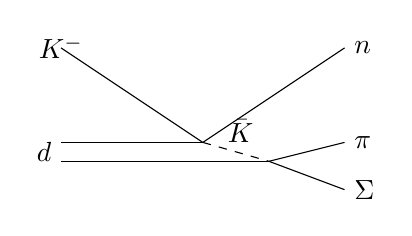
\begin{tikzpicture}[scale=1.2]
      \draw (-1.5,    1) node {$K^-$}--(0,    0);
      \draw (-1.5,    0)--(0,    0);
      \draw (-1.5, -0.2)--(0.7, -0.2);
      \node (d) at (-1.5, -0.1) [left] {$d$};
      
      \draw (0, 0) -- (0.7, -0.2) [dashed];
      \node (barK) at (0.4, -0.1) [above] {$\bar{K}$};
      
      \draw ( 1.5,  -0.5) node [right] {$\Sigma$} -- (0.7, -0.2);
      \draw ( 1.5,  -0.0) node [right] {$\pi$}    -- (0.7, -0.2);
      \draw ( 1.5,  1.0) node [right] {$n$}      -- (0,    0);
    \end{tikzpicture}
    %% \caption{
    %%   The diagram of 2step $K^- d \rightarrow n \pi \Sigma$ reaction.
    %% }
    %% \label{fig:kd_2step}
  \end{figure}
  \vspace{-1cm}
  
  \begin{align*}
    \frac{d^2}{dM_{\pi\Sigma}}{d\Omega_n}
    &=\bra{n \pi \Sigma} T^2_{\bar{K}N_2 \rightarrow \pi \Sigma} G_0(\bar{K}) T^1_{K^- N_1 \rightarrow \bar{K} n} \ket{K^- d}\\
    &=\int T^2_{\bar{K}N_2 \rightarrow \pi \Sigma} G_0(\bar{K}) T^1_{K^- N_1 \rightarrow \bar{K}n } \Phi_{d}(p_{N_1}) dp_{N_1}
  \end{align*}

  {
    \small
    $\Phi_{d}(p)$ : Fermi motion of deuteron. \\
    $T^1_{K^- N \rightarrow \bar{K} n}$ : $T$-matrix of 1step $K^- N \rightarrow \bar{K} n$.\\
    $G_0(\bar{K})$ : Green fuction of intermediate $\bar{K}$.\\
    $T^2_{\bar{K}N \rightarrow \pi \Sigma}$ : $T$-matrix of 2step $\bar{K}N \rightarrow \pi \Sigma$.\\

  }
  
\end{frame}
